\section{The Oculomotor System} \label{sec:bt_TheOculomotorSystem}

Only second to the brain, the human eye is one of the most complex organs in our bodies. Its anatomy has perplexed scientists for centuries, and the mere fact of its complexity was an essential argument that Charles Darwin had to circumvent during the making of \textit{On The Origin of Species} (\cite{oyster1999}). "If a complex mechanical contrivance like a watch requires a watchmaker, something as wonderful as the eye, which is beyond the wit and ability of a man to create, must have an eye maker." 

What Darwin struggled to explain in 1859 is better understood in today's academic community, and it is apparent that vision has proved a winning factor in evolution. Zoologists believe that animals, where eyes have developed beyond a primitive stage, constitute about 96\% of known living species. Human eyes are inherited from our primate ancestors, and little has changed in terms of general eye composition since we diverged from our most common ancestors about 30 million years ago. The versatility of the human eye in combination with our brain has been one of the driving forces of our rapid cultural evolution. This thesis is chiefly concerned with the oculomotor system, an intricate network of muscles and neural circuits that control eye position and, in turn, determine how humans perceive their environment.
% The final 4\% can be found in environments where light is nonexistent, or in immobile animals where relocation as a response to the detection of light poses no real advantage. This suggests that 

\subsection{Brief Anatomy}
The oculomotor system can not be explained in detail by its components alone. The human eye incorporates several distinct major and minor structures and regions that transform light into perception. However, its macroscopic anatomy is quite simple and readily explainable. As Gordon Walls, a renowned professor of physiological optics and optometry, once put it: "The eye is (simply) a fluid-filled chamber enclosed by three coats or layers, of tissue. It is an optical system made of leather, water and jelly" (\cite{oyster1999}), as can be observed by figure \ref{fig:bt_eye}.

Leather would refer to the white \textit{sclera}, a rigid tissue making up most of the outer coat of the eye. The gel-like \textit{vitreous} is what makes up most of the interior volume. Light is admitted through and partially refracted by an area at the front of the eye, where the sclera yields to a transparent coat termed the \textit{cornea}. After the cornea, light passes through an aperture stop known as the \textit{pupil}. The pupil is essentially just an opening within the \textit{iris}, a sphincter known for its abundance of melatonin pigments and rich colors. Its purpose is to regulate the pupil opening. Light is further refracted in the \textit{lens} before reaching the \textit{retina} at the very back of the eye. Here, the light is processed by millions of hypersensitive photoreceptor cells and transferred to the brain. 

\begin{figure}[h]
    \centering
    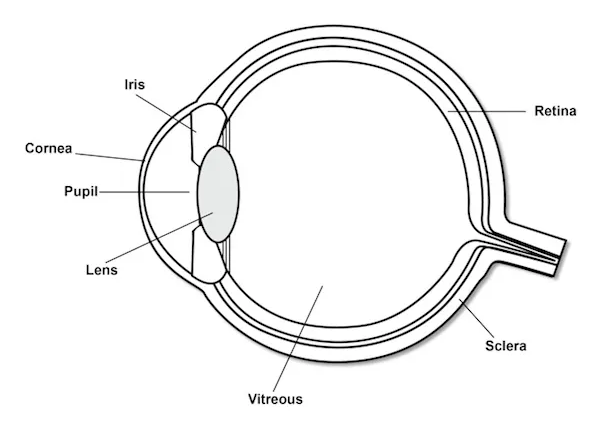
\includegraphics[width=0.8\textwidth]{Images/bt_eye.png}
    \caption{Anatomy of the human eye, in terms of its major and most structures.}
    \label{fig:bt_eye}
\end{figure}

\subsubsection{The Extraocular Muscles}

Central to the oculomotor system are the muscles that allow for physical translation and rotation of the eye in space, enabling the brain to control which parts of the environment it wants to perceive. Movement is enabled by \textit{extraocular} muscles arranged in three agonist-antagonist pairs, meaning there are six in total, each pulling in the opposite direction of another. Together, they allow for accurate vertical and lateral positioning and -90\degree to +90\degree torsions. Muscle fibers are inherently elastic, and each extraocular muscle exerts passive force even when not actively engaged. This elasticity means that for the eye to hold any stationary position, all six muscles are counterbalanced by an equal and opposite force, producing an equilibrium.

% A set of extraocular muscle lengths dictates any particular eye position. which in turn is dictated a set of \textit{innervational} commands from the neural circuitry that controls eye movement. For a muscle fiber, its innervation level corresponds to the steady-state firing rate of the neural signals to its muscle neuron. 

%Innervation, the process of supplying nerve signals to an organ or part of the body. A particular level of innervation to a muscle always produces the same state of contraction or relaxation and a particular set of innervational commands to the six muscles always produces the same eye position relative to all three axes of rotation.

% As we know from mechanics, the acceleration of an object is given by the net sum of its acting forces. As such, the speed of eye movement is given by the change in innervation of the extraocular muscles from one level to another. Slow eye movements can be recognized by gradual changes of a neuron's mean firing rate. Fast movements require a brief high-velocity burst of neural activity which initiates the rapid movement.  As will be made clear in the following subsection, the human eye is capable of a very wide range of movement velocities, from 0.05\degree to 500\degree per second. Such an enormous range of contraction velocities make the extraocular muscles unique compared to any other muscles in our bodies.

%The speed of eye movement is dictated the change in innervation of the extraocular muscles from one level to another. Every level of innervation in turn dictated by the steady-state firing rate of nerve impulses from each muscles motor nerve. Slow eye movements (e.g. smooth pursuit) can be recognized by gradual changes of a neuron's mean firing rate. Fast movements (saccades) require a brief high-frequency burst of neural activity that produce forces which initiates the rapid eye movement.

\subsection{Eye Movement}
Since most retina photoreceptors are concentrated at the fovea, a minuscule 1.5mm wide pit right behind the lens, only a tiny area in the field of view provides clear vision. Interestingly, the brain dedicates about 25\% of the visual cortex to processing information from the fovea (\cite{hubel1974}). Therefore, as we will see, eye movements are crucial to moving the field of view between areas of interest. Other reasons are image stabilization, focus, and more. This importance gives rise to the need for complex eye movement patterns, some of which will be mentioned here.

Whenever attention is shifted from one point to the next, a \textit{saccade} event occurs. These are typically between 30-80ms in duration and can reach velocities of up to 500\degree/s (\cite{holmqvist2011}). Although the eye is not particularly heavy (7.5g in adults), its mass does pertain to a tiny bit of inertia which resists movement. Additionally, since its primary interior and cornea are made of a gel-like substance, most saccadic events are followed by a "wobbling." These \textit{post-saccadic oscillation} have durations of 10-30ms.

% Vision supression during saccadic motion? 
% - file:///C:/Users/joste/Personal/Uni/9_Semester/TTK4550_Fordypningsprosjekt/Papers/Unread/Land,%20Furneaux%20(1997),%20Oculomotor%20system.pdf
% - file:///C:/Users/joste/Personal/Uni/9_Semester/TTK4550_Fordypningsprosjekt/Papers/Unread/Judge%20et.al%20(1980),%20Vision%20during%20saccadic%20eye%20movements.pdf
% - file:///C:/Users/joste/Personal/Uni/9_Semester/TTK4550_Fordypningsprosjekt/Papers/Unread/Campbell,%20Wurtz%20(1978),%20Saccadic%20omission.pdf

Perhaps one of the most discussed events in eye movement research, along with saccades, are \textit{fixations} and they occur whenever the user is focusing attention on one particular point. The fixation duration is usually tens or a few hundred milliseconds but can last for several seconds at most. During this time, the extraocular muscles will move the eye in very small \textit{microsaccades} and \textit{drifts} around the point of fixation. These micro-movements require sensitive equipment to detect and are no more than rapid, high-frequency flicks of about 0.2\degree of arc. Although seemingly erratic, these movements are critical for vision, as a fully stabilized image on the retina will eventually fade and disappear. What we perceive as vision is essentially a series of very rapid after-images, sort of similar to that produced by a camera flash.

One final eye movement type is called the \textit{smooth pursuit} and is in some ways similar to the saccade in how it moves the eye in one continuous motion. Functionally, however, the movement is driven by a completely different part of the brain. As its name suggests, it can be classified by much smoother motions than the saccade, with velocities between 10-30\degree/s and arbitrary durations. They occur only when the eyes actively follow a moving target or conversely when fixating on a stationary object while the head or body is moving. The reader is encouraged to attempt such a movement themselves, perhaps when looking at a plain, white wall. They are likely to realize that without such "triggers," it is impossible to produce a smooth pursuit forcibly.

% \textit{The overlapping fields of view of two eyes. Constitute vergence, another eye movement type which is necessary to place objects in plane of focus. Slow movements, up to 30 \degree/s. Under everyday conditions, other eye movements are generally superimposed on vergences.}
% }








